% \subsection{Notes}
% \begin{enumerate}
%     \item Motivate The Problem Cosmo
%     \item Introduce The Theory Cosmo + Lensing
%     \item Explain How Theory Solves The Problem
%     \item Current Results/ Experiments
%     \item Explain Problems with WeakLensing
%     \item Summarise
% \end{enumerate}

% Discuss probing the large scale universe with CMB, supernvae, clustering
% and lensing. 
% Note weak lensing makes no assumptions about the nature of dark matter
% and no assumptions about relationship between visible matter and mass therefore
% it provides a directly measured mass distribution in the universe as a function of 
% redshift. Therefore we can get info on DE and DM directly. It is sensitive to intial
% conditions so it can even give info on inflation. 
\subsection{Standard Model of Cosmology}

The fundamental assumption in cosmology, known as the cosmological principle, is that we live in a homogenous (independent of position) and isotropic (independent of direction) universe \cite{general_2013,ryden}. Solving Einstein's equations under the geometric symmetries provided by the cosmological principle and taking into account the expansion of the universe one finds that the dynamics of the universe are governed by the Friedman equation \cite{ryden,general_2013},

\begin{equation}
  H^2(z) = H_0^2 \left(\Omega_r (1+z)^4 + \Omega_m (1+z)^3 + \Omega_k (1+z)^2 + \Omega_\Lambda \frac{\rho_\Lambda(z)}{\rho_\Lambda(0)}\right)
  \label{eq:friedman}
\end{equation}


Remeber to show the Standard Model parameters! can be found in wikipedia.
\par Angular diameter distance is the one of relvance in lensing (distance measures in cosmology)
Distances in cosmo \cite{Hogg:1999ad}
lol  

% \begin{enumerate}
%   \item Motivation (modified gravity vs Dark energy) is DE constant in space ? and time ?
%   \item FRW Standard Cosmology 
%   \item Distance Measures In Cosmo
%   \item Gravitational Evolution of Dark matter
%   \item Observables and Parameters
% \end{enumerate}
\subsubsection{Matter Power Spectrum}
\cite{extragalactic}

\subsection{Bending of Light}
The fundamental concept on which weak lensing is built is gravity's ability to alter the path of a photon. This phenomenon is explored in full detail in \cite{GR1,basicLens,Mellier:1998pk}.
In this subsection I present a simple overview of the theory behind the bending of light necessary to develop the weak lensing formalism. For more detailed calculations consult \cite{GR1,basicLens,Mellier:1998pk}.
\subsubsection{Newtonian Lens}
\label{subsec:newtonlens}

It is a common misconception that the gravitational bending of light is an exclusive property of GR.
However, gravity induced alterations to a photon's path are predicted by newtonian mechanics \cite{lensingbook}. To illustrate this 
consider a mass $M$ located at the origin of the cartesian plane and a corpuscle(newtonian photon) 
propagating along the $x=b$ line (in this context $b$ is known as the impact parameter). 
Newton's second law predicts that the presence of the point mass will result in a momentum transfer
between the two objects. If the corpuscle starts with 
momentum $(p,0)$ then it will end up with momentum $(p_x,p_y)$.
Therefore, the particle path is deflected by some angle $\hat{\alpha}$. The deflection angle is 
simply given by 

\begin{equation}
  \sin(\hat{\alpha}) = \frac{p_y}{\sqrt{p_x^2+p_y^2}}
  \label{deflectionnewton}
\end{equation}


\par For very small deflections we have $p\approx p_x >> p_y$ and $\hat{\alpha} << 1$. 
Therefore \autoref{deflectionnewton} simplifies to $\hat{\alpha}
\approx \frac{p_y}{p_x}$. We now consider the infinitesimal deflection along the entire path of the photon with
$d\hat{\alpha} = \frac{dp_y}{p_x} = \frac{1}{px} dx \frac{dp_y}{dx}$. Therefore, we can find the deflection
angle by 

\begin{equation}
  \begin{split}
  \hat{\alpha}_N &= -\frac{1}{p_x} \int dx \frac{dp_y}{dx} \\
  &= -\frac{1}{cp_x} \int dx \frac{dp_y}{dt}  \\ 
  &= \frac{2GM}{c^2b}
  \end{split}  
  \label{newtonbend}
\end{equation}

We note that the mass of the corpuscle cancels out of the deflection equation. Therefore this equation applies
for massless particles i.e. photons. Therefore \autoref{newtonbend} provides a newtonian description for the 
bending of light \cite{lensingbook}.

\subsubsection{General Relativistic Bending of Light}
The Einstein's field equations in the presence of a charge free static point mass is uniquely solved by 
the Schwarzchild metric \cite{GR1}. The Schwarzchild metric is

\begin{equation}
  ds^2 = \left ( 1-\frac{r_s}{r} \right )  dt^2 - \left( 1-\frac{r_s}{r}\right) ^{-1} dr^2 -r^2 d\Omega^2
  \label{schwarz}
\end{equation}

where $r_s$ is the Shcwarzchild radius of the system given by $r_s=2 \mu = 2GM/c^2$ and $(t,r,\Omega)$ are the standard parameters for 4D space-time in polar coordinates. We can analyze the path of the photon from \autoref{subsec:newtonlens} by studying the geodesic equations of the metric and finding the conserved
quantities of the system. We can then combine the conservation equations with the tangent vector norm condition for a 
null path to get the shape equation of the system as 

\begin{equation}
  \frac{d\phi}{dr} = \frac{1}{r^2} \left(\frac{1}{b^2}- \frac{1}{r^2} \left(1-\frac{2\mu}{r}\right) \right)^{-1/2}
  \label{shapeeqbend}
\end{equation}

where $(r,\phi)$ are the photons position in 2D polar coordinates and $b$ is the impact parameter. Rewriting this equation
under the transformation of $r = 1/u$ and working pertrubatively around $u(\mu =0) = \frac{1}{b}\sin \phi
$ we get 

\begin{equation}
  u(\phi) \approx \frac{1}{b}\sin \phi + \frac{3\mu}{2b^2} \left(1+\frac{1}{3}\cos 2 \phi \right)
  \label{eq:pertshape}
\end{equation}

in the limit were $\phi << 1$ and $u \rightarrow 0$ \autoref{eq:pertshape} simplifies to $\phi = \hat{\alpha}_N =\frac{2GM}{c^2b} $. Geometrically the deflection is given by $\hat{\alpha}= 2\phi$ and therefore the deflection angle is

\begin{equation}
  \hat{\alpha} = 2\hat{\alpha}_N=\frac{4GM}{c^2b}
  \label{grbend}
\end{equation}

We conclude that general relativity predicts a factor of 2 greater deflection form a point mass than is predicted by newtonian mechanics. This relationship greatly simplifies the formalism developed for weak lensing. 

\subsection{Weak Lensing Formalism}
Now that we have a theoretical understanding of the Cosmological parameters we would like to measure, as well as an understanding of how gravitational fields impact the trajectory of light. We are ready to develop the theoretical formalism on which all weak lensing applications are built. This formalism is based on a combination of the frameworks developed in these sources \cite{basicLens,general_2013,rachel_2018,hoekstra,massey_2013,Mellier:1998pk,Hoekstra:2013gua}.

\subsubsection{Weak thin lens}
\begin{figure}
  \begin{center}
    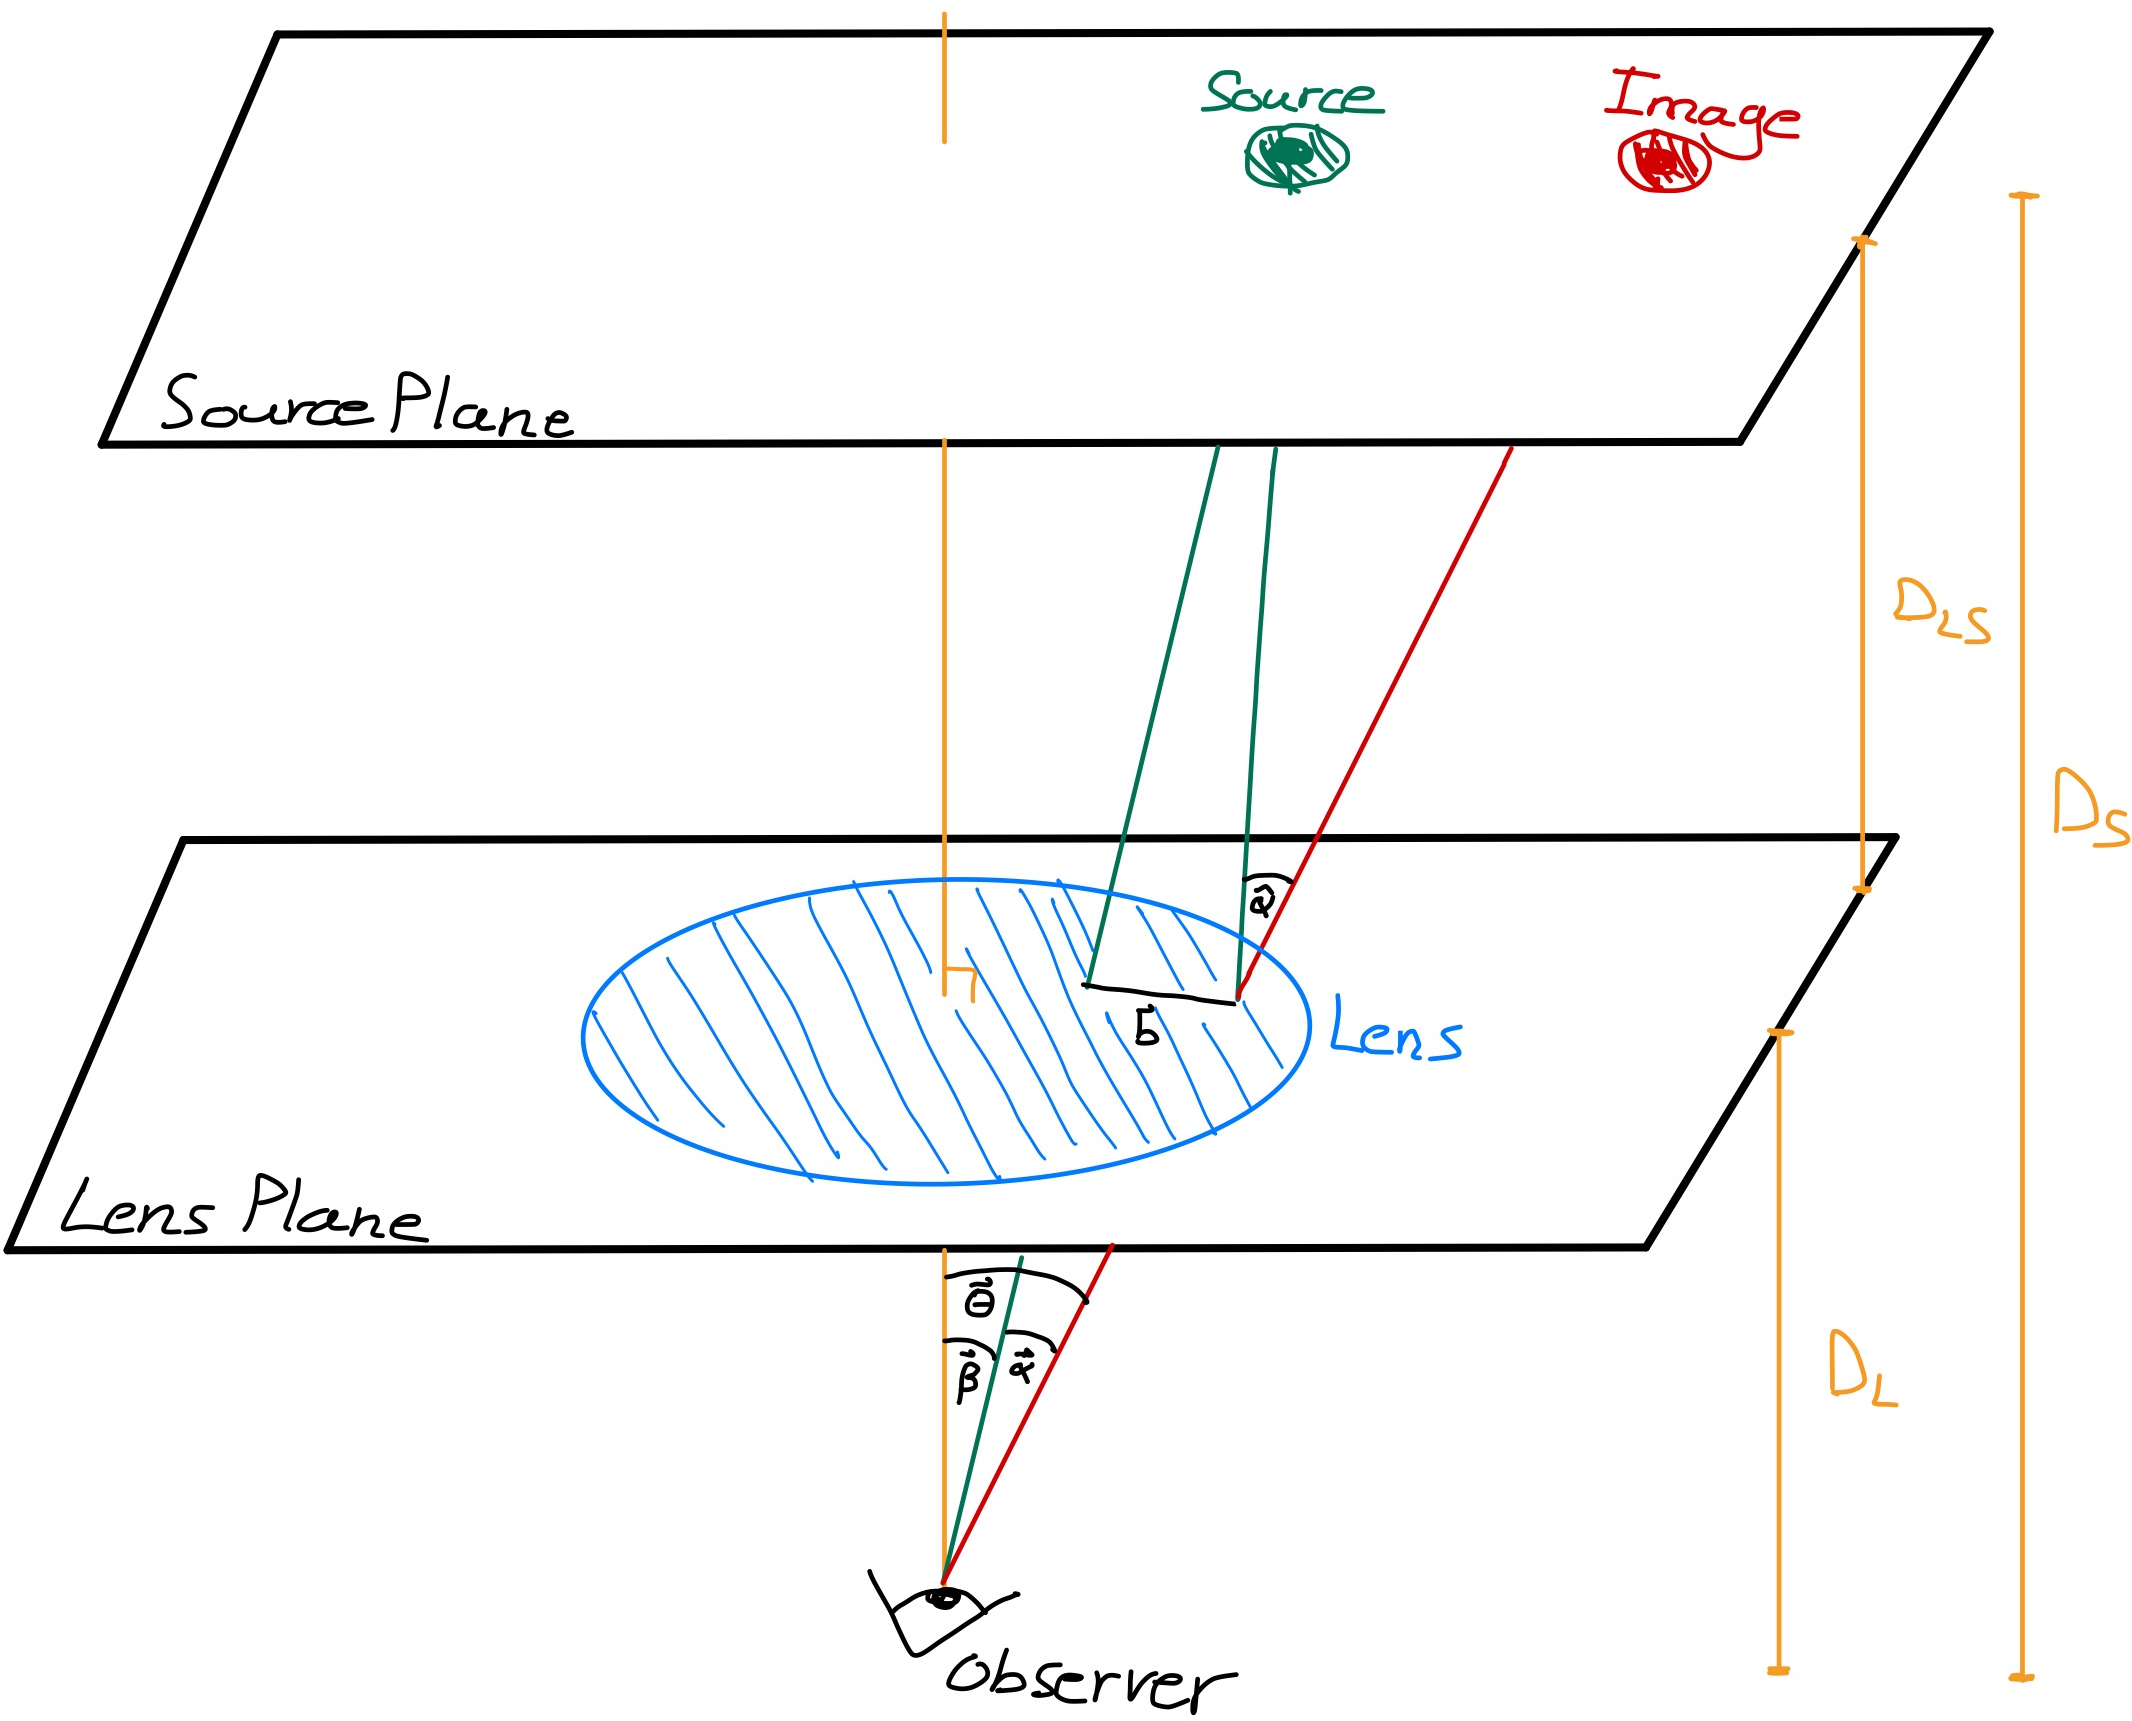
\includegraphics[width=\textwidth]{figs/lens.jpg}
  \end{center}
  \caption{Sketch of a thin lens system highlighting the parameters of relevance in the weak lensing formalism. It is conventional to assume the planes are orthogonal to the z axis.}
  \label{fig:lens}
\end{figure}
In order to develop our formalism let us consider a general lensing system as seen in \autoref{fig:lens}. For astronomical applications on cosmological scales the distance from the observer to the lens $D_L$, the distance from the lens to the source $D_{LS}$, and the distance from the observer to the source $D_S$ are much greater than the thickness of the lens along the optical axis. Therefore we can treat the lens as a "thin lens", i.e. it lives on a planar slice (lensing plane) along the line of sight. We project the mass and potential of the lens onto the lensing plane by defining the projected surface density $\Sigma$ and projected potential $\Phi$ as

\begin{equation}
  \begin{split}
    \Sigma(x,y) &= \int \rho(x,y,z) dz \\
    \Phi &= \int \phi dz
  \end{split}
  \label{eq:surfacedensity+surfacepot}
\end{equation}

were $\rho$ and $\phi$ are the spatial mass density and the newtonian potential respectively. We can now use the results from the previous section to find the deflection angle $\hat{\alpha}$ due to the extended thin lens. The deflection is given by

\begin{equation}
  \hat{\alpha} = \frac{2}{c^2} \nabla \Phi(x,y)
  \label{eq:deflectionthinlens}
\end{equation}

were the factor of 2 comes from \autoref{grbend} and $\nabla$ is the two dimensional gradient. Note that this equation is equivalent to that describing the deflection of light by an optical lens with refractive index $n=1-2\phi/c^2$, hence the name lensing. Geometrically we have $\beta = \theta - \alpha$ and $\hat{\alpha} = \frac{D_{LS}}{D_S}\alpha$ from \autoref{fig:lens}. This leads us to the ray trace equation

\begin{equation}
  \beta = \theta - \frac{D_{LS}}{D_S} \hat{\alpha}(\theta)
  \label{eq:raytrace}
\end{equation}

The ray trace equation is the fundamental equation in weak lensing relating all the geometric properties of the system to one another. 

\subsubsection{Differential deflection of adjacent light rays}
In the weak limit the actual deflections are not observable because the true position of the source is unknown. As a result, only the effects of differential deflection can be measured. Two adjacent light rays from the source pass through the lens at slightly different positions and will therefore be deflected differently. This effect results in a remapping of the observed surface brightness of the source $I_s$ to the observed surface brightness $I_{obs}$. This mapping can be linearized and is therefore given by 

\begin{equation}
  I_{obs}(\vec{\theta}) \approx I_s(A\vec{\theta})
  \label{eq:linearizedbright}
\end{equation}

were $A$ is the Jacobian of the transformation. A convenient convention is to rewrite the 2D Jacobian as 

\begin{equation}
  A = \delta_{ij} - \frac{\partial^2 \Phi}{\partial \theta_i \partial \theta_j} =  \begin{pmatrix}
    1-\kappa-\gamma_+ & -\gamma_\times \\
    -\gamma_\times & 1-\kappa+\gamma_+
    \end{pmatrix}
  \label{eq:Ajacobian}
\end{equation}

were we have defined the convergence $\kappa$ shear $\gamma = \gamma_+ + i \gamma_\times$ as 

\begin{equation}
  \begin{split}
   \kappa &= \frac{1}{2}(\partial_x^2 \Phi + \partial_y^2 \Phi)\\
   \gamma_+ &=  \frac{1}{2}(\partial_x^2 \Phi - \partial_y^2 \Phi)\\
   \gamma_\times &=  \partial_x \partial_y \Phi \\
  \end{split}
  \label{eq:kappagamma}
\end{equation}

We can now study the geometric implications of the remapping. If we consider a circular source we see that  $\gamma_+$ and $\gamma_\times$ correspond to a stretching of the circle along the x/y axis and the x=y line respectively, $\kappa$ corresponds to isotropic enlargement of the source's profile, and since the mapping conserves surface brightness we observe an increase of the total flux by a magnification factor

\begin{equation}
  \mu = \frac{1}{\text{det}A} = \frac{1}{(1-\kappa)^2 - \gamma_+^2 - \gamma_\times^2}
  \label{eq:magnificaiton}
\end{equation}

these geometric effects are illustrated in \autoref{fig:shears}. To be more specific a circular source is mapped to an ellipse with major axis $a = (1-\kappa - |\gamma|)^{-1}$ and minor axis $b = (1-\kappa + |\gamma|)^{-1}$ \cite{massey_2013}. If we define the reduced shear as $g = \gamma / (1-\kappa)$ then an ellipse with ellipticity $\epsilon_{orig}$ is mapped to an ellipse with ellipticity $\epsilon_{obs}$ given by 

\begin{equation}
  \epsilon_{obs} = \frac{\epsilon_{orig} + g}{1+g^* \epsilon_{orig}} \approx \epsilon_{orig} + \gamma
  \label{eq:ellip}
\end{equation}

the approximate relationship is a result of the weak limit ($\kappa << 1$). \autoref{eq:ellip} and \autoref{eq:kappagamma} demonstrate that by measuring the apparent shapes of lensed objects we are measuring information about the lensing potential and hence the matter overdensity \cite{rachel_2018,Hoekstra:2013gua,hoekstra}. \autoref{eq:ellip} indicates that a population of intrinsically round sources ($\epsilon_{orig}=0$) would be ideal, but unfortunately real  galaxies  have  an  average  intrinsic ellipticity of 0.25 per component \cite{Hoekstra:2013gua}. Instead the lensing signal is inferred by averaging over an ensemble of sources, under the assumption that the unlensed orientations are random \cite{rachel_2018,Hoekstra:2013gua}. In the next section we talk about how such measurements are made.

\begin{figure}
    \begin{center}
      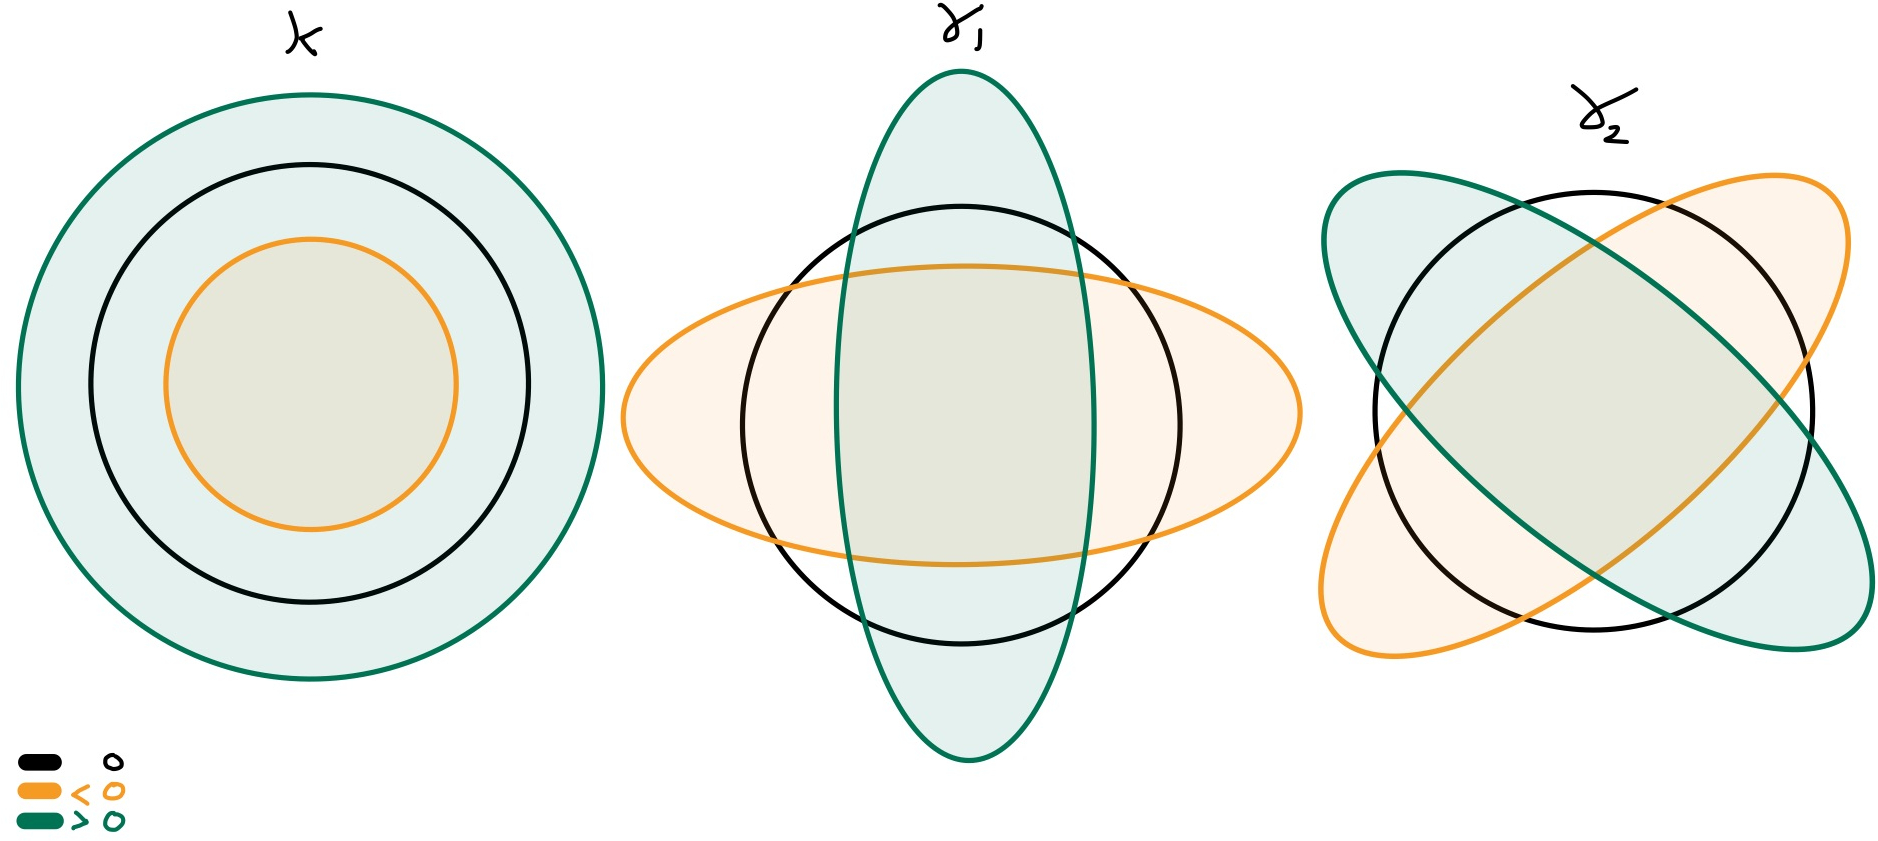
\includegraphics[width=\textwidth]{figs/shear-11.jpg}
    \end{center}
    \caption{The effects of the convergence $\kappa$ and  the shear $\gamma$ on a circular image of a galaxy. The black line represents the nominal image, orange represents positive parameter values, and green represents negative parameter values.}
    \label{fig:shears}
\end{figure}
